% --- Page Style ---
\settasks{label-width=4.6em, item-indent=4.6em}
\pagestyle{fancy}
\fancyhf{}
\lhead{Algebra --- Unit 7}
\rhead{Exam ID: \underline{\hspace{2cm}}}
\lfoot{Show all work. No calculators unless stated.}
\rfoot{Page \thepage}
\renewcommand{\headrulewidth}{0.4pt}
\renewcommand{\footrulewidth}{0.4pt}

% --- Header spanning both columns ---
\twocolumn[
  \begin{center}
    {\huge \textbf{Unit 7 Test}} \\
    \vgap
    {\large \textbf{Algebra}} \\
    \vgap
    \begin{tabular}{|l|l|}
      \hline
      \textbf{Student Name:} & \hspace{6cm} \\ \hline
      \textbf{Date:} & \hspace{6cm} \\ \hline
    \end{tabular}
  \end{center}
  \vgap
  \textbf{Instructions:} Show all work. If an expression is undefined, explain your reasoning.
  \vgap
]

% % --- Form A ---
% \section*{Form A}

% \begin{enumerate}[leftmargin=*, label=\textbf{\arabic*.}]

%   \item Given $f(x) = -2\sin\bigl(\dfrac{\pi}{3}x - 2\bigr) + 4$, indicate each of the following. \points{1} each

%   \begin{center}
%   \small
%   \begin{tabular}{|l@{\quad}l|}
%   \hline
%   Domain: & \blank[3em] \\
%   Range: & \blank[3em] \\
%   Period: & \blank[3em] \\
%   Amplitude: & \blank[3em] \\
%   Coordinates of Relative Maxima: & \blank[4em] \\
%   $x$-intercept(s): & \blank[4em] \\
%   \hline
%   \end{tabular}
%   \end{center}
%   \vgapp

%   \item Graph $f(x) = -\dfrac{1}{2}\cos\bigl(\dfrac{x}{2} + \dfrac{\pi}{2}\bigr) - 2$. Show at least one period. \points{4}

%   \begin{center}
%   \begin{tikzpicture}[x=0.35cm, y=0.35cm, line cap=round, line join=round]
%     \draw[thick,->] (-2,0) -- (8,0) node[right] {$x$};
%     \draw[thick,->] (0,-4) -- (0,2) node[above] {$y$};
%     \foreach \x in {-2,0,2,4,6,8} \draw (\x,2pt) -- (\x,-2pt) node[below,font=\scriptsize] {\x};
%     \foreach \y in {-4,-2,0,2} \draw (2pt,\y) -- (-2pt,\y) node[left,font=\scriptsize] {\y};
%     \draw[gray!40] (-2,-4) grid[step=1] (8,2);
%   \end{tikzpicture}
%   \end{center}
%   \vgapp

%   \item Graph $f(x) = -2\csc(\pi x - 2\pi) - 3$. Show at least one period. \points{4}

%   \begin{center}
%   \begin{tikzpicture}[x=0.4cm, y=0.25cm, line cap=round, line join=round]
%     \draw[thick,->] (-1,0) -- (5,0) node[right] {$x$};
%     \draw[thick,->] (0,-8) -- (0,2) node[above] {$y$};
%     \foreach \x in {0,1,2,3,4} \draw (\x,2pt) -- (\x,-2pt) node[below,font=\scriptsize] {\x};
%     \draw[gray!40] (-1,-8) grid[step=1] (5,2);
%   \end{tikzpicture}
%   \end{center}
%   \vgapp

%   \item A period of $p(x) = -3\cot\bigl(\dfrac{\pi x}{7} - 1\bigr) + 3$ is shown below. If $B$ has coordinates $(h, k)$ and $0 \le h \le 7$, find: \points{1} each

%   Period of $p(x)$: \blank

%   All vertical asymptotes of $p(x)$: \blank

%   All Points of Inflection: \blank

%   Coordinates of A: \blank

%   Coordinates of B: \blank

%   Coordinates of C: \blank
%   \vgappp

%   \item Given $f(x) = -2\sec\bigl(4x - \dfrac{\pi}{11}\bigr) + 8$, indicate each of the following. \points{1} each

%   \begin{center}
%   \small
%   \begin{tabular}{|l@{\quad}l|}
%   \hline
%   Domain: & \blank[3em] \\
%   Range: & \blank[3em] \\
%   Period: & \blank[3em] \\
%   Amplitude: & \blank[3em] \\
%   State 4 different Vertical Asymptote(s): & \blank[5em] \\
%   Coordinates of all relative minima: & \blank[5em] \\
%   \hline
%   \end{tabular}
%   \end{center}
%   \vgapp

%   \item How many times does $\cos(600x) = -\dfrac{1}{3}$ on the interval $\bigl(0, \dfrac{\pi}{6}\,\bigr]$? \points{1}
%   \vgappp

%   \item State the domain and range of each function. \points{1} per row

%   \begin{center}
%   \small
%   \begin{tabular}{|l@{\quad}l@{\quad}l|}
%   \hline
%   $f(x)$ & Domain & Range \\
%   \hline
%   $\operatorname{arcsec}(x)$ & \blank[2.5em] & \blank[2.5em] \\
%   $\arccos(x)$ & \blank[2.5em] & \blank[2.5em] \\
%   $\arctan(x)$ & \blank[2.5em] & \blank[2.5em] \\
%   \hline
%   \end{tabular}
%   \end{center}
%   \vgapp

%   \item Evaluate each. If no real value exists, write undefined and explain. \points{2} each

%   $\sin\bigl(-2\arccos\bigl(-\dfrac{1}{2}\bigr)\bigr)$: \blank

%   $\tan(\operatorname{arccsc}(2))$: \blank

%   $\cos\bigl(\arcsin\bigl(\dfrac{\pi}{2}\bigr)\bigr)$: \blank

%   $\cot\bigl(\operatorname{arcsec}\bigl(\dfrac{6}{5}\bigr)\bigr)$: \blank
%   \vgappp

%   \item The expression $\tan\bigl(\arccos\bigl(-\dfrac{13}{5}\bigr)\bigr)$ has no real value but has a complex value. Find that complex value. \points{2}
%   \vgappp

% \end{enumerate}

% \clearpage
% % --- Form B ---
% \section*{Form B}

% \begin{enumerate}[leftmargin=*, label=\textbf{\arabic*.}, resume]

%   \item Given $f(x) = -3\cos\bigl(\dfrac{\pi}{3}x - 5\bigr) + 4$, indicate each of the following. \points{1} each

%   \begin{center}
%   \small
%   \begin{tabular}{|l@{\quad}l|}
%   \hline
%   Domain: & \blank[3em] \\
%   Range: & \blank[3em] \\
%   Period: & \blank[3em] \\
%   Amplitude: & \blank[3em] \\
%   Coordinates of Relative Minima: & \blank[4em] \\
%   $x$-intercept(s): & \blank[4em] \\
%   \hline
%   \end{tabular}
%   \end{center}
%   \vgapp

%   \item Graph $f(x) = -2\sin\bigl(\dfrac{x}{2} + \dfrac{\pi}{4}\bigr) - 2$. Show at least one period. \points{4}

%   \begin{center}
%   \begin{tikzpicture}[x=0.35cm, y=0.35cm, line cap=round, line join=round]
%     \draw[thick,->] (-2,0) -- (8,0) node[right] {$x$};
%     \draw[thick,->] (0,-6) -- (0,2) node[above] {$y$};
%     \foreach \x in {-2,0,2,4,6,8} \draw (\x,2pt) -- (\x,-2pt) node[below,font=\scriptsize] {\x};
%     \foreach \y in {-6,-4,-2,0,2} \draw (2pt,\y) -- (-2pt,\y) node[left,font=\scriptsize] {\y};
%     \draw[gray!40] (-2,-6) grid[step=1] (8,2);
%   \end{tikzpicture}
%   \end{center}
%   \vgapp

%   \item Graph $f(x) = 2\sec\bigl(\dfrac{\pi}{2}x - \pi\bigr) - 3$. Show at least one period. \points{4}

%   \begin{center}
%   \begin{tikzpicture}[x=0.4cm, y=0.25cm, line cap=round, line join=round]
%     \draw[thick,->] (-1,0) -- (5,0) node[right] {$x$};
%     \draw[thick,->] (0,-6) -- (0,4) node[above] {$y$};
%     \foreach \x in {0,1,2,3,4} \draw (\x,2pt) -- (\x,-2pt) node[below,font=\scriptsize] {\x};
%     \draw[gray!40] (-1,-6) grid[step=1] (5,4);
%   \end{tikzpicture}
%   \end{center}
%   \vgapp

%   \item A period of $p(x) = -6\cot\bigl(\dfrac{\pi x}{3} - 5\bigr) + 3$ is shown below. If $B$ has coordinates $(h, k)$ and $0 \le h \le 3$, find: \points{1} each

%   Period of $p(x)$: \blank

%   All vertical asymptotes of $p(x)$: \blank

%   All Points of Inflection: \blank

%   Coordinates of A: \blank

%   Coordinates of B: \blank

%   Coordinates of C: \blank
%   \vgappp

%   \item Given $f(x) = -2\sec\bigl(7x - \dfrac{\pi}{3}\bigr) + 18$, indicate each of the following. \points{1} each

%   \begin{center}
%   \small
%   \begin{tabular}{|l@{\quad}l|}
%   \hline
%   Domain: & \blank[3em] \\
%   Range: & \blank[3em] \\
%   Period: & \blank[3em] \\
%   Amplitude: & \blank[3em] \\
%   State 4 different Vertical Asymptote(s): & \blank[5em] \\
%   Coordinates of all relative minima: & \blank[5em] \\
%   \hline
%   \end{tabular}
%   \end{center}
%   \vgapp

%   \item How many times does $\sin(800x) = \dfrac{1}{6}$ on the interval $\bigl(0, \dfrac{\pi}{4}\,\bigr]$? \points{1}
%   \vgappp

%   \item State the domain and range of each function. \points{1} per row

%   \begin{center}
%   \small
%   \begin{tabular}{|l@{\quad}l@{\quad}l|}
%   \hline
%   $f(x)$ & Domain & Range \\
%   \hline
%   $\operatorname{arcsec}(x)$ & \blank[2.5em] & \blank[2.5em] \\
%   $\arcsin(x)$ & \blank[2.5em] & \blank[2.5em] \\
%   $\arctan(x)$ & \blank[2.5em] & \blank[2.5em] \\
%   \hline
%   \end{tabular}
%   \end{center}
%   \vgapp

%   \item Evaluate each. If no real value exists, write undefined and explain. \points{2} each

%   $\cos\bigl(-2\arcsin\bigl(-\dfrac{1}{2}\bigr)\bigr)$: \blank

%   $\cot(\operatorname{arcsec}(2))$: \blank

%   $\cos\bigl(\arcsin\bigl(\dfrac{\pi}{3}\bigr)\bigr)$: \blank

%   $\cot\bigl(\operatorname{arcsec}\bigl(-\dfrac{7}{4}\bigr)\bigr)$: \blank
%   \vgappp

%   \item The expression $\cot\bigl(\arccos\bigl(-\dfrac{13}{12}\bigr)\bigr)$ has no real value but has a complex value. Find that complex value. \points{2}
%   \vgappp

% \end{enumerate}

% \clearpage
% % --- Form C ---
% \section*{Form C}

% \begin{enumerate}[leftmargin=*, label=\textbf{\arabic*.}, resume]

%   \item Given $f(x) = -2\sin\bigl(\dfrac{\pi}{6}x + 3\bigr) - 34$, indicate each of the following. \points{1} each

%   Domain: \blank

%   Range: \blank

%   Period: \blank

%   Amplitude: \blank

%   Coordinates of Relative Maxima: \blank

%   $x$-intercept(s): \blank
%   \vgapp

%   \item Graph $f(x) = -\dfrac{1}{2}\cos\bigl(\dfrac{x}{2} - \dfrac{3\pi}{2}\bigr) - 2$. Show at least one period. \points{4}

%   \begin{center}
%   \begin{tikzpicture}[x=0.35cm, y=0.35cm, line cap=round, line join=round]
%     \draw[thick,->] (-2,0) -- (8,0) node[right] {$x$};
%     \draw[thick,->] (0,-6) -- (0,2) node[above] {$y$};
%     \foreach \x in {-2,0,2,4,6,8} \draw (\x,2pt) -- (\x,-2pt) node[below,font=\scriptsize] {\x};
%     \foreach \y in {-6,-4,-2,0,2} \draw (2pt,\y) -- (-2pt,\y) node[left,font=\scriptsize] {\y};
%     \draw[gray!40] (-2,-6) grid[step=1] (8,2);
%   \end{tikzpicture}
%   \end{center}
%   \vgapp

%   \item Graph $f(x) = -2\sec(\pi x - 3\pi) - 3$. Show at least one period. \points{4}

%   \begin{center}
%   \begin{tikzpicture}[x=0.4cm, y=0.25cm, line cap=round, line join=round]
%     \draw[thick,->] (-1,0) -- (5,0) node[right] {$x$};
%     \draw[thick,->] (0,-8) -- (0,2) node[above] {$y$};
%     \foreach \x in {0,1,2,3,4} \draw (\x,2pt) -- (\x,-2pt) node[below,font=\scriptsize] {\x};
%     \draw[gray!40] (-1,-8) grid[step=1] (5,2);
%   \end{tikzpicture}
%   \end{center}
%   \vgapp

%   \item A period of $p(x) = 7\tan\bigl(\dfrac{\pi x}{6} - 5\bigr) - 23$ is shown below. If $B$ has coordinates $(h, k)$ and $0 \le h \le 6$, find: \points{1} each

%   Period of $p(x)$: \blank

%   All vertical asymptotes of $p(x)$: \blank

%   All Points of Inflection: \blank

%   Coordinates of A: \blank

%   Coordinates of B: \blank

%   Coordinates of C: \blank
%   \vgappp

%   \item Given $f(x) = -5\csc\bigl(3x - \dfrac{2\pi}{13}\bigr) + 8$, indicate each of the following. \points{1} each

%   Domain: \blank

%   Range: \blank

%   Period: \blank

%   Amplitude: \blank

%   State 4 different Vertical Asymptote(s): \blank

%   Coordinates of all relative minima: \blank
%   \vgapp

%   \item How many times does $\sin(1200x) = \dfrac{1}{5}$ on the interval $\bigl(0, \dfrac{\pi}{3}\,\bigr]$? \points{1}
%   \vgappp

%   \item State the domain and range of each function. \points{1} per row

%   \begin{center}
%   \small
%   \begin{tabular}{|l@{\quad}l@{\quad}l|}
%   \hline
%   $f(x)$ & Domain & Range \\
%   \hline
%   $\operatorname{arccsc}(x)$ & \blank[2.5em] & \blank[2.5em] \\
%   $\arccos(x)$ & \blank[2.5em] & \blank[2.5em] \\
%   $\operatorname{arccot}(x)$ & \blank[2.5em] & \blank[2.5em] \\
%   \hline
%   \end{tabular}
%   \end{center}
%   \vgapp

%   \item Evaluate each. If no real value exists, write undefined and explain. \points{2} each

%   $\sin\bigl(-2\arccos\bigl(\dfrac{1}{2}\bigr)\bigr)$: \blank

%   $\sec(\operatorname{arccsc}(2))$: \blank

%   $\cos\bigl(\arcsin\bigl(\dfrac{2\pi}{3}\bigr)\bigr)$: \blank

%   $\csc\bigl(\arctan\bigl(\dfrac{6}{5}\bigr)\bigr)$: \blank
%   \vgappp

%   \item The expression $\tan\bigl(\arccos\bigl(-\dfrac{5}{3}\bigr)\bigr)$ has no real value but has a complex value. Find that complex value. \points{2}
%   \vgappp

% \end{enumerate}

% \clearpage
% % --- Form D ---
% \section*{Form D}

\begin{enumerate}[leftmargin=*, label=\textbf{\arabic*.}, resume]

  \item Given $f(x) = 3\cos\bigl(\dfrac{\pi}{4}x + 1\bigr) - 2$, indicate each of the following. \points{1} each

  \begin{center}
  \small
  \begin{tabular}{|l@{\quad}l|}
  \hline
  Domain: & \blank[3em] \\
  Range: & \blank[3em] \\
  Period: & \blank[3em] \\
  Amplitude: & \blank[3em] \\
  Coordinates of Relative Maxima: & \blank[4em] \\
  $x$-intercept(s): & \blank[4em] \\
  \hline
  \end{tabular}
  \end{center}
  \vgapp

  \item Graph $f(x) = 2\sin\bigl(\dfrac{x}{3} - \dfrac{\pi}{6}\bigr) + 1$. Show at least one period. \points{4}

  \begin{center}
  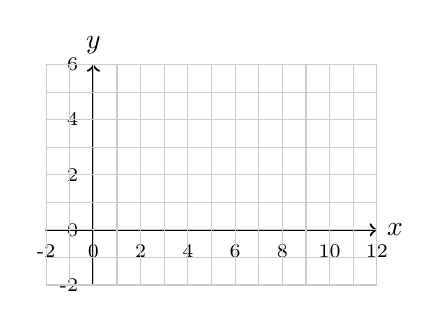
\begin{tikzpicture}[x=0.3cm, y=0.35cm, line cap=round, line join=round]
    \draw[thick,->] (-2,0) -- (12,0) node[right] {$x$};
    \draw[thick,->] (0,-2) -- (0,6) node[above] {$y$};
    \foreach \x in {-2,0,2,4,6,8,10,12} \draw (\x,2pt) -- (\x,-2pt) node[below,font=\scriptsize] {\x};
    \foreach \y in {-2,0,2,4,6} \draw (2pt,\y) -- (-2pt,\y) node[left,font=\scriptsize] {\y};
    \draw[gray!40] (-2,-2) grid[step=1] (12,6);
  \end{tikzpicture}
  \end{center}
  \vgapp


  \newpage
  \item Graph $f(x) = -3\csc(2\pi x) + 2$. Show at least one period. \points{4}

  \begin{center}
  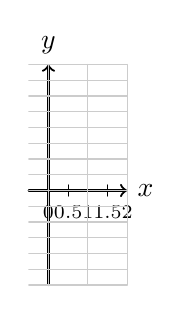
\begin{tikzpicture}[x=0.5cm, y=0.2cm, line cap=round, line join=round]
    \draw[thick,->] (-0.5,0) -- (2,0) node[right] {$x$};
    \draw[thick,->] (0,-6) -- (0,8) node[above] {$y$};
    \foreach \x in {0,0.5,1,1.5,2} \draw (\x,2pt) -- (\x,-2pt) node[below,font=\scriptsize] {\x};
    \draw[gray!40] (-0.5,-6) grid[step=1] (2,8);
  \end{tikzpicture}
  \end{center}
  \vgapp

  \item A period of $p(x) = -4\tan\bigl(\dfrac{\pi x}{5} - 2\bigr) + 1$ is shown below. If $B$ has coordinates $(h, k)$ and $0 \le h \le 5$, find: \points{1} each

  Period of $p(x)$: \blank

  All vertical asymptotes of $p(x)$: \blank

  All Points of Inflection: \blank

  Coordinates of A: \blank

  Coordinates of B: \blank

  Coordinates of C: \blank
  \vgappp


  \newpage
  \item Given $f(x) = 3\sec\bigl(5x - \dfrac{\pi}{7}\bigr) - 4$, indicate each of the following. \points{1} each

  \begin{center}
  \small
  \begin{tabular}{|l@{\quad}l|}
  \hline
  Domain: & \blank[3em] \\
  Range: & \blank[3em] \\
  Period: & \blank[3em] \\
  Amplitude: & \blank[3em] \\
  State 4 different Vertical Asymptote(s): & \blank[5em] \\
  Coordinates of all relative minima: & \blank[5em] \\
  \hline
  \end{tabular}
  \end{center}
  \vgapp

  \item How many times does $\cos(400x) = \dfrac{2}{5}$ on the interval $\bigl(0, \dfrac{\pi}{8}\,\bigr]$? \points{1}
  \vgappp

  \item State the domain and range of each function. \points{1} per row

  \begin{center}
  \small
  \begin{tabular}{|l@{\quad}l@{\quad}l|}
  \hline
  $f(x)$ & Domain & Range \\
  \hline
  $\operatorname{arcsec}(x)$ & \blank[2.5em] & \blank[2.5em] \\
  $\operatorname{arccsc}(x)$ & \blank[2.5em] & \blank[2.5em] \\
  $\operatorname{arccot}(x)$ & \blank[2.5em] & \blank[2.5em] \\
  \hline
  \end{tabular}
  \end{center}
  \vgapp


  \newpage
  \item Evaluate each. If no real value exists, write undefined and explain. \points{2} each

  $\tan\bigl(2\arcsin\bigl(\dfrac{3}{5}\bigr)\bigr)$: \blank

  $\sin\bigl(\arccos\bigl(-\dfrac{2}{3}\bigr)\bigr)$: \blank

  $\sec\bigl(\operatorname{arccsc}\bigl(\dfrac{5}{4}\bigr)\bigr)$: \blank

  $\cot\bigl(\arctan\bigl(-\dfrac{12}{5}\bigr)\bigr)$: \blank
  \vgappp

  \item The expression $\cot\bigl(\arccos\bigl(-\dfrac{8}{5}\bigr)\bigr)$ has no real value but has a complex value. Find that complex value. \points{2}
  \vgappp

  \item \textbf{(Advanced)} A sinusoidal function $f(x) = A\sin(Bx - C) + D$ has range $[-5, 1]$, period $6$, and no horizontal shift (i.e., a maximum occurs at $x = 0$). Find the exact values of $A$, $B$, $C$, and $D$. \points{4}
  \vgappp


  \newpage
  \item \textbf{(Advanced)} Find all $x$ in $[0, 2\pi)$ such that $$\sin\bigl(2\arccos(x)\bigr) = \dfrac{1}{2}.$$ (First express $\arccos(x)$ in terms of $x$ and then solve.) \points{4}
  \vgappp

  \item \textbf{(Advanced)} Simplify to a single algebraic expression in $x$ (no trig or inverse trig): $\cos\bigl(2\arctan(x)\bigr)$. Show work. \points{3}
  \vgappp

\end{enumerate}
